I first probed for injections by the GC like those that were seen during the DDoS attack on GitHub.
Failing to find any, I turned my attention to other JavaScript files that the GC may be intercepting and replacing with malicious substitutes.
\subsection{GitHub DDoS}
This experiment looked for GC packets as were observed during the DDoS on GitHub.
The observation specifically was a modified JavaScript file upon request for \texttt{hm.baidu.com/h.js}, an analytics tracking script similar to that used by Google Analytics.
The URI also has a site-specific query appended.
For example, the analytics tracking script for the site \texttt{7k7k.com} is \texttt{http://hm.baidu.com/\allowbreak h.js?4f1beaf39805550dd06b5cac412cd19b}
The unmodified script for this same site can be found here: \url{https://github.com/tagatac/ttlprobe/blob/prelim/h.js}.
According to \mbox{NETRESEC}~\cite{Hjelmvik2015}, the modified file contains some obfuscated code that sends requests to GitHub in a 2-second loop.
Marczak et al. calculated that the substitution is made 1.75\% of the time, as long as your IP address is not ignored by the GC altogether, which happened to one of the machines they used for probing~\cite{Marczak2015}.
I ran a Python script (\url{https://github.com/tagatac/ttlprobe/blob/prelim/falunjs.py}) to download the analytics script for \texttt{7k7k.com} 1000 times.
MD5 hashes of every file match that of the unmodified JavaScript.
This provides some evidence to support the hypothesis that the GC is no longer responding to queries for \texttt{hm.baidu.com/h.js}.
\subsection{Other JavaScript Files}\label{otherjs}
What about other JS files?
Is the GC responding to requests for other JS files with malicious substitutions?
In order to answer this question, I gathered URIs for many JavaScript files from several of the most-visited sites in China.
I then requested each of these files several times, varying the TTL value of the request until I could identify the minimum TTL value required (the minimum distance the request needed to travel along the path to the hosting server) in order for the server to send me the file.
This experiment consisted of six main pieces:
\begin{enumerate}\addtolength{\itemsep}{-.35\baselineskip}
	\item gathering the list of most-visited sites in China,
	\item choosing a DNS server,
	\item crawling the most-visited sites for JavaScript file URIs,
	\item identifying a proper timeout to use when requesting the URIs,
	\item estimating the distance to each domain hosting one or more of the JS files, and
	\item identifying the minimum request TTL value required to obtain each JS file.
\end{enumerate}
The remainder of \autoref{otherjs} discusses the implementation of these pieces in further detail.
\subsubsection{The Most-visited Sites in China}\label{alexa}
\texttt{Alexa.com} was chosen as the source for the list of most-visited sites in China~\cite{AlexaCN}.
A simple web crawler constructed on top of the Scrapy web crawling framework~\cite{Scrapy} was used to scrape the list of the top 500 most-visited and most-viewed sites: \url{https://github.com/tagatac/ttlprobe/blob/master/crawler/crawler/spiders/alexa.py}.
The crawler visits each of the pages in the Alexa top sites list, and records the domain names of all 25 sites listed on each of the 20 pages, for a total of 500 domain names.
Using the built-in Scrapy pipeline system, these domain names are written to a file in JSON format.
This crawler took 493 milliseconds to run.
\subsubsection{DNS Servers}\label{dns}
As mentioned earlier, U.S.-based DNS servers often resolve Chinese domains (like many of those obtained by the crawler in \autoref{alexa}) to servers outside of mainland China (e.g. in Hong Kong).
In order to maximize the likelihood of the TTL probes passing through the GC infrastructure, I preferred a Chinese DNS server that would resolve Chinese domains to servers inside mainland China.
I visited the same list of public Chinese DNS servers used in \autoref{gfwtls}~\cite{PublicDNS} and chose the most reliable 9 out of the most recently checked 100 servers.
To decide which was most suitable for this experiment, I analyzed each of these servers for its location, performance as measured with \texttt{namebench}~\cite{Stromberg2010}, and the location of the server to which it resolves \texttt{www.baidu.com} (Table \ref{tab_dns}).
An OpenDNS server was also analyzed for comparison.
For all of the following experiments, the two fastest DNS servers which place \texttt{www.baidu.com} in mainland China were used (\texttt{118.194.196.109} and \texttt{114.112.79.22}).
\begin{table}
	\footnotesize
	\begin{tabular}{ | p{0.7in} | p{0.4in} | p{0.4in} | p{0.4in} | p{0.4in} | }
	\hline
	\textbf{Server \allowbreak{}Address} & \textbf{Location} & \textbf{Mean \allowbreak{}Response Time (ms)} & \textbf{Fastest \allowbreak{}Response Time (ms)} & \textbf{Baidu \allowbreak{}Location} \\ \hline
	\hline
	208.67.222.222 & San Fran., US & 32.1 & 1.1 & Central District, HK \\ \hline
	103.7.5.13 & Laohekou, China & 344.51 & 205.2 & Central District, HK \\ \hline
	192.151.227.196 &  & 398.68 & 222.2 & Central District, HK \\ \hline
	118.194.196.109 & Beijing, China & 559.77 & 241.5 & Beijing, China \\ \hline
	114.112.79.22 & Beijing, China & 608.10 & 216.0 & Beijing, China \\ \hline
	124.254.1.114 & Beijing, China & 632.41 & 217.2 & Beijing, China \\ \hline
	61.182.80.61 & Shijia\-zhuang, China & 685.63 & 225.9 & Beijing, China \\ \hline
	202.202.24.65 & Chong\-qing, China & 942.96 & 229.8 & Nanjing, China \\ \hline
	112.95.147.99 & Shenzhen, China & ---\tablefootnote{replica of 192.151.227.196} & --- & Central District, HK \\ \hline
	159.226.223.193 & Beijing, China & ---\tablefootnote{failed the namebench correctness tests} & --- & Beijing, China \\ \hline
	\end{tabular}
	\caption{
		Performance and location details for several Chinese DNS servers obtained from a list of public servers~\cite{PublicDNS} (compared to one OpenDNS server), ordered by mean response time.
		``Baidu Location'' refers to the location of the server returned by a lookup query for \texttt{www.baidu.com}.
		The two fastest servers which place \texttt{www.baidu.com} in mainland China were \texttt{118.194.196.109} and \texttt{114.112.79.22}.
	}
	\label{tab_dns}
\end{table}
\subsubsection{JavaScript URIs}\label{jsfiles}
Using the list of domain names obtained with the crawler described in \autoref{alexa}, two other crawlers were written to scrape Javascript URIs from each domain.
The first only scrapes JS URIs from the homepage of each domain: \url{https://github.com/tagatac/ttlprobe/blob/master/crawler/crawler/spiders/homepages.py}.
The second attempts to crawl the entire site for each domain, scraping JS URIs from each page in each domain: \url{https://github.com/tagatac/ttlprobe/blob/master/crawler/crawler/spiders/topchinese.py}.
\subsubsection*{Homepages-only Crawler}\label{homepages-crawler}
The first crawler visits each of the domains obtained from the Alexa top 500 list, and performs a regular expression search on the source of the entire homepage for JS file URIs.
The regular expression used is \texttt{https?://[URI\_CHARS]*\textbackslash{}.js\allowbreak{}(?:\textbackslash{}?[URI\_CHARS?]*)?}, where \texttt{URI\_CHARS} is the set of valid URI characters, except for question marks, which can only be used in the query and fragment, and single quotes, which are rarely used in URIs and cause issues for parsing.
Using the built-in Scrapy pipeline system, these URIs are written, along with the \texttt{referer} URL to a file in JSON format.
Note that both crawlers may record any given script URI more than once, as the scraping records (referer, URI) pairs.

After setting the system DNS servers to those identified in \autoref{dns}, this crawler ran to completion in 8 minutes and 32 seconds, gathering 3,427 (referer, JavaScript file URI) pairs from 374 of the 500 homepages.
Of the 3,427 (referer, URI) pairs, 2,757 correspond to unique URIs.
The JS files are hosted across 737 domains.
The crawler encountered 106 Scrapy exceptions, of which 60 were timeout errors, 37 were DNS errors, and 9 were no-response errors.
3 more errors were caused by a Scrapy bug wherein an exception is raised when TLS certificates fail verification~\cite{Calderone2015}.
\subsubsection*{Full-site Crawler}\label{full-crawler}
The second crawler performs a much broader crawl.
It visits the homepage of each of the domains obtained from the Alexa top 500 list, like the homepages-only crawler, scraping for JS URIs in the same way with the same regular expression.
However, this crawler also gathers all of the hyperlinks (using Scrapy's link-gathering library), and visits all of those links provided they are also within the list of top 500 domains.
Again, it scrapes each of these pages for JS URIs and hyperlinks to visit, and recurses.

I have never seen this crawler complete.
A first run, performed in the default depth-first order, and storing links to visit in memory, gathered 910,490 JS (referer, JS file URI) pairs from 268,537 distinct pages before running out of memory and crashing after 19 hours and 1 minute.
These files are hosted on 118 different domains.
The domain which accounted for the largest fraction of the JS URIs was \texttt{cmsjs.eastmoney.com}, hosting 377,156 of the 0.9M (referer, URI) pairs, of which only 640 of the URIs are unique.
This large number of repeated URIs is not unexpected because this run scraped in DFO, often recording the same JS file URIs for many similar pages on the same domain.
This run also used a more basic regular expression for extracting URIs, one which ignores the queries and segments (everything after the first question mark).

A second run, performed in breadth-first order, and storing link to visit on disk, has been running since 1am on August 16\textsuperscript{th}.
At the time of writing this, 2pm on September 1\textsuperscript{st}, this second run has gathered 27,836,060 (referer, JS file URI) pairs from 2,977,239 distinct pages.
These files are hosted on 4,908 different domains.
The domain which so far accounts for the largest fraction of the JS URIs is \texttt{static-web.b5m.com}, hosting 6,421,586 of the 27.8 million (referer, URI) pairs.
\subsubsection{Proper Timeouts}
In order to identify the minimum request TTL value required to obtain each JS file (discussed further in \autoref{distance-ttl}), it will be necessary to make several requests for each file, varying the TTL value associated with those requests.
Furthermore, to identify the \textit{minimum} TTL value required to obtain these files, it will be necessary to issue several requests which will \textit{not} obtain each file.
As such, a performance bottleneck in this probe will be time spent waiting for responses which will -- by design -- never come.
It is therefore important to choose a suitable timeout for this waiting -- one which minimizes the amount of unnecessary waiting without giving up so soon that a significant number of responses is ignored.

To this end, I wrote a Python 3 script to time the downloading of a sample of the JS files for which I obtained URIs in \autoref{jsfiles}: \url{https://github.com/tagatac/ttlprobe/blob/master/timeouttest.py}.
This script chooses at random a specified number (100 by default) of JS URIs from a results file generated by one of the crawlers.
It then parses that URI for the scheme, hostname, and request.
Using that information, it generates an HTTP request message to look as if it is originating from a current version of Chrome.
Finally, it issues the request using the Python 3 socket library (and ssl library if necessary), starts a timer, receives the response, and stops the timer.
Each file in the randomly-selected list is requested thrice, and the response time for each request is recorded.
Running this script for 100 URIs from the DFO partial results of the full-site crawler descibed in \autoref{jsfiles}, showed that the average response time was 718 milliseconds, with a standard deviation of 2,798 milliseconds.
The maximum response time was 47.3 seconds; however, 99\% of the file responses were received within 3 seconds of the request.
For this reason, 3 seconds was the time chosen to stop waiting for a response after issuing a \texttt{GET} request for one of the JS files.
\subsubsection{Distance to Servers \& Minimum TTL Values}\label{distance-ttl}
Finally, the most important part of the GC probe is the probe itself.
The distance to the hosting servers and the minimum TTL values required to obtain JS files from those servers are both determined within the same Python 3 script: \url{https://github.com/tagatac/ttlprobe/blob/master/gcprobe.py}.
This script first sorts the JS files to be probed by domain, allowing the probes to be parallelized by domain.
It then spawns a thread pool with up to 512 threads and a results file lock, and allows each thread to probe the list of files hosted by a single domain.
The probe for each domain involves:
\begin{itemize}\addtolength{\itemsep}{-.35\baselineskip}
	\item resolving the IP address for the domain via the DNS servers from \autoref{dns},
	\item performing a TCP traceroute with \texttt{scapy-python3}~\cite{Dobelis2015} (very similar to \texttt{tcptraceroute}) on the domain to estimate the distance to its servers, and
	\item for each (referer, URI) pair for which the file identified by the URI is hosted by the domain:
	\begin{enumerate}
		\item Set an upper bound on the minimum TTL required to download the file (initially three more than the distance estimated by the traceroute).
		\item Set a lower bound on the TTL required (initially zero).
		\item\label{loop} Request the file five times with a TTL halfway between the lower bound and the upper bound, and with headers that look like the request is coming from a current version of Chrome.
		\item If the file is received following any of the five requests, set the upper bound to be the TTL used.
			If not, set the lower bound to be one greater than the TTL used.
		\item\label{ttl} Repeat from \ref{loop} until the lower bound is the same as the upper bound.
			This is decidedly the minimum TTL required to download this file.
		\item Record the script URI, the \texttt{referer} URL, the traceroute result for the domain, the TTL value obtained in \ref{ttl}, the difference between the traceroute result and the TTL value, and whether the script was actually downloaded or not.
			(It may not be if it is not received by a request with TTL set to the initial upper bound.)
		\item If the difference between the traceroute result and the TTL value is greater than 3, save the response to a file for further analysis.
			(This may be a malicious injection by an entity other than the targeted server, which has been estimated to be further away than the request should have reached.)
	\end{enumerate}
\end{itemize}
\subsection{Testing the Probe}\label{testing}
Before placing too much stock in the results of the probe script, I demonstrated that it was able to identify files injected in a controlled environment in a manner similar to that of the GC's injections.
\subsubsection{Network Architecture}
The test probe was run from a Debian 8 virtual machine ``TTLProbe'' hosted in VMware on my desktop computer.
All of the virtual machine's traffic was routed through its only network interface (on a local VMware network) to another Debian 8 virtual machine ``Router'', also hosted in VMware on my desktop, by setting Router as its gateway in \texttt{/etc/network/interfaces}.
In addition to a network interface on the same local VMware network with TTLProbe, Router had another network interface bridged to the physical Wi-Fi interface on my desktop, giving it access to the Internet.
Router was then configured with \texttt{iptables}~\cite{Russell2000} to allow forwarding of IPv4 packets, thus giving TTLProbe access to the Internet.
\subsubsection{File Injection}
In addition to IPv4 forwarding, however, Router was further configured with \texttt{iptables} to respond to HTTP requests for a specific file: \texttt{http://adnetpub.yaolan.com/js/adpubs.js}.
This is accomplished as follows:
\begin{enumerate}\addtolength{\itemsep}{-.35\baselineskip}
	\item\label{synack} All TCP SYN-ACK packets forwarded from \texttt{http://adnetpub.yaolan.com} (117.79.133.119:80) to the host-only network are queued for inspection with the \texttt{NFQUEUE} target.
	\item All TCP packets destined for \texttt{http://adnetpub.yaolan.com:80} from TTLProbe are analyzed with the \texttt{strings} netfilter extension for requests for \texttt{http://adnetpub.yaolan.com/js/\allowbreak{}adpubs.js}.
	\item If \texttt{adpubs.js} is requested, the packet is also queued for inspection with the \texttt{NFQUEUE} target, although using a different queue than in step~\ref{synack}.
	\item Finally, a Python 2 daemon processes both queues using \texttt{python-netfilterqueue}~\cite{Kerkhoff2015}, Python bindings for the \texttt{libnetfilter\_queue} C library:
	\begin{itemize}
		\item The SYN-ACK packets are inspected for their sequence numbers, and then accepted, so that they continue on the TTLProbe, allowing TCP connections to be made.
		\item The request packets are dropped so that the request never makes it to \texttt{adnetpub.yaolan.com}.
		\item Then a phony JS file containing a reference to a fake URI at \texttt{malice.com} is used to construct a TCP packet in response to the request, and the sequence number from above is used to make it look like the packet is part of the same TCP connection.
	\end{itemize}
\end{enumerate}
Figure~\ref{fig_testnetwork} is a simple diagram of the network layout.
\begin{figure}
	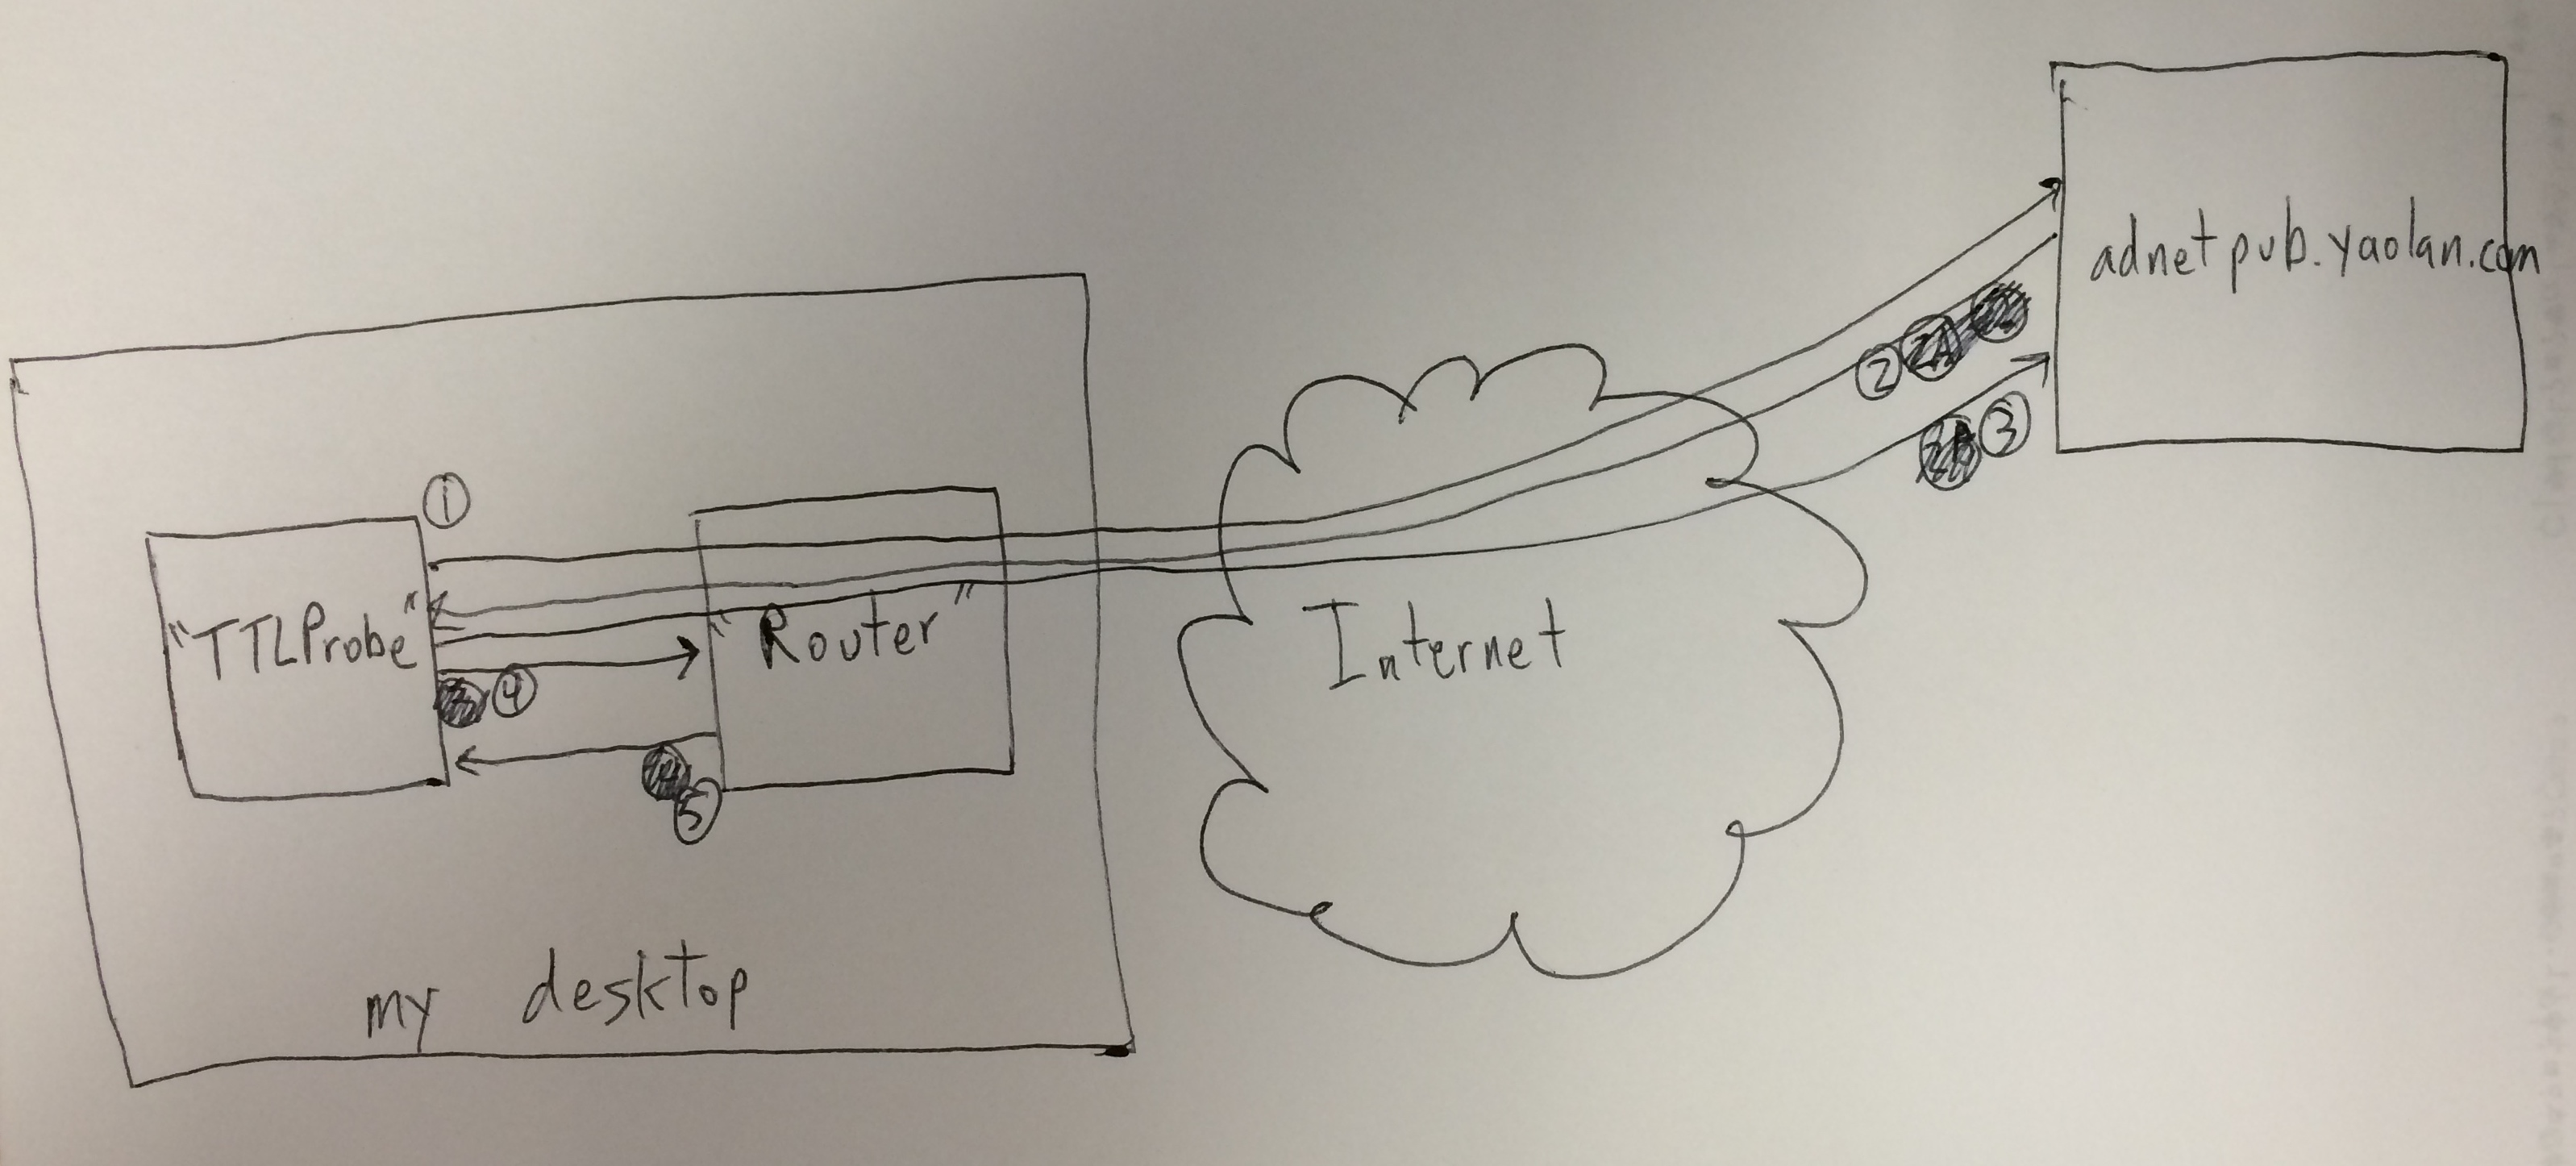
\includegraphics[width=\columnwidth]{figures/testnetwork}
	\captionsetup{singlelinecheck=off}
	\caption[asdf]{
		A diagram of the five packets involved in an injection of the file \texttt{http://adnetpub.yaolan.com/js/adpubs.js}.
		\begin{enumerate}\addtolength{\itemsep}{-.35\baselineskip}
			\item TTLProbe sends a TCP SYN packet to \texttt{http://adnetpub.yaolan.com} via its IP address 117.79.133.119:80 through Router.
			\item \texttt{adnetpub.yaolan.com} replies with a SYN-ACK packet through Router.
				Router's \texttt{iptables} are configured such that this packet is inspected before forwarding for the TCP sequence number.
			\item TTLProbe sends an ACK packet to \texttt{http://adnetpub.yaolan.com} to complete the TCP connection.
			\item TTLProbe requests the file \texttt{http://adnetpub.yaolan.com\allowbreak{}/js/adpubs.js} from \texttt{http://adnetpub.yaolan.com} through Router.
				However, Router does not forward this packet to \texttt{http://adnetpub.yaolan.com}, but drops it instead.
			\item Finally, Router sends a phony JS file back to TTLProbe.
		\end{enumerate}
	}
	\label{fig_testnetwork}
\end{figure}
Requests for the file from \texttt{wget}, \texttt{netcat}, and the TTL probe script developed in this work are all able to receive the phony JS file as if it had come from \texttt{adnetpub.yaolan.com}.
\subsubsection{Verdict}
The probe was run on a small subset of the URIs scraped by the homepage-only crawler described in \autoref{homepages-crawler} -- particularly those scripts scraped from one homepage: \texttt{http://www.yaolan.com}.
As expected, the GC probe script detected the injection of the single file \texttt{http://adnetpub.yaolan.com/js/adpubs.js} as coming from somewhere much closer than the server hosting it.
In fact, Figure~\ref{fig_histtest} shows that it was the only file to differ from the traceroute distance estimate at all, and in dramatic fashion.
\begin{figure}
	\includegraphics[width=\columnwidth]{figures/histtest}
	\caption{
		A histogram showing how often a file request succeeded with a TTL value less than the number of hops to the server (as estimated by the traceroute), when downloading a small subset of files from URIs scraped by the homepage-only crawler.
		Note the single file for which the TTL value was less than the number of hops to the server, was the very file that the VM Router was injecting.
	}
	\label{fig_histtest}
\end{figure}
This result gives us some confidence that the probe script is able to detect files injected between the computer running it the servers hosting the files it requests.